%\section{Multitask learning for cold-start playlist recommendation}
%\section{Multitask learning for playlist recommendation}
%\section{Recommending playlists via multitask learning}
\section{Recommending playlist via multitask learning}
%\section{Playlist recommendation via multitask learning}
\label{sec:method}

\begin{figure*}[!t]
    \centering
    \begin{subfigure}[t]{2.3in}
        \centering
        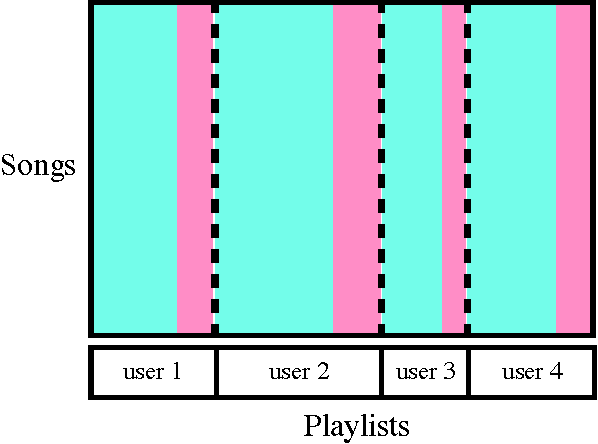
\includegraphics[height=1.6in]{fig/cp.pdf}
        \caption{Cold Playlists}
    \end{subfigure}
    \begin{subfigure}[t]{2.3in}
        \centering
        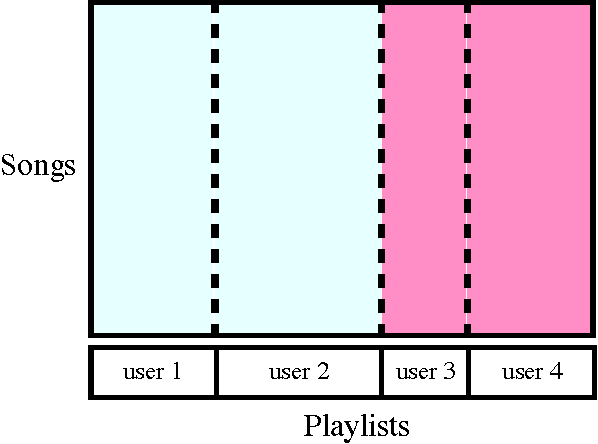
\includegraphics[height=1.6in]{fig/cu.pdf}
        \caption{Cold Users}
    \end{subfigure}
    \begin{subfigure}[t]{2.3in}
        \centering
        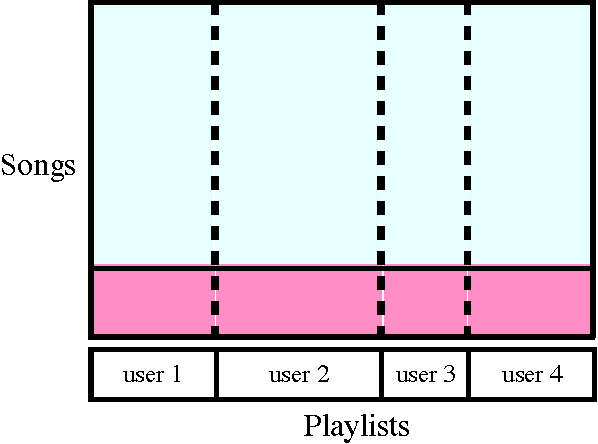
\includegraphics[height=1.6in]{fig/cs.pdf}
        \caption{Cold Songs}
    \end{subfigure}
    %\caption{Three cold-start settings: training set (cyan), test set (magenta)}
	\caption{Three settings of cold-start playlist recommendation.
In each setting,
rows represent songs, and a column represents a playlist, 
which is a binary vector where an element denotes if the corresponding song is in the playlist.
%Playlists are first grouped by user, then split into training (Cyan) and test set (Magenta).
%(a) Cold Playlists: a portion of playlists from each user are held for test
%See text below for description.
Playlists are grouped by user.
{\color[rgb]{.4,1,1} \bf Light Cyan} represents playlists or songs in the training set, and
{\color[rgb]{1,0,.5} \bf dark Magenta} represents playlists or songs in the test set.
{\bf (a) Cold Playlists}: recommending personalised playlists (Magenta) for each user 
given users' existing playlists (Cyan); 
%by learning from her existing playlists (Cyan); 
{\bf (b) Cold Users}: recommending playlists for new users (Magenta) 
given playlists from existing users (Cyan);
%by learning playlists from existing users (Cyan); 
%by learning playlists from existing users (Cyan); 
{\bf (c) Cold Songs}: recommending newly released songs (Magenta) to extend users' existing playlists (Cyan).
}
\label{fig:setting}
\end{figure*}


%- multitask learning problem
%- solutions for three cold-start settings
%- learning parameters by minimising bipartite ranking loss
%- constrained optimisation formulation
%- unconstrained optimisation of classification loss

We first describe the three cold-start settings considered in the paper,
%In this section, 
%we introduce a multitask objective that supports the three cold-start settings described in Section~\ref{sec:problem}. 
%we describe a multitask learning method that works in all three cold-start settings introduced in previous sections.
%We consider %the problem of 
then formulate
playlist recommendation as a multitask learning problem, 
where each task involves recommending a set of songs given a user or playlist.
We propose to optimise a bipartite ranking loss that encourages songs in a playlist
to be ranked higher than those are not.
%
This results in a convex %constrained 
optimisation problem with an enormous number of constraints.
By exploiting an equivalence between bipartite ranking and binary classification,
we efficiently approximate an optimal solution by minimising an unconstrained classification loss.

%We exploit an equivalence between bipartite ranking and binary classification to 
%avoid dealing with an enormous number of constraints 
%We formulate a convex constrained optimisation problem for this multitask learning 

%We optimise the multitask learning objective by minimising a bipartite ranking loss that encourages songs in a playlist
%to be ranked higher than those are not, which involves a convex constrained optimisation problem.
%By exploiting an equivalence relationship between bipartite ranking and binary classification, 
%we can approximate an optimal solution of the constrained optimisation problem by minimising a classification loss without any constraints.
%This enables efficient optimisation of the multitask learning objective.

%Inspired by an equivalence relationship between bipartite ranking and binary classification, 
%we show that an optimal solution of this problem can be approximated by minimising a classification loss without any constraints,
%which enables efficient optimisation of the multitask objective.

%We propose to approximate an optimal solution by minimising a classification loss.
%we propose a classification loss that approximates the multitask objective without %dealing with 
%any constraints, which enables efficient optimisation of the multitask objective.
%This enables the efficient optimisation of the multitask objective.

%We propose a ranking approach to optimise the multitask objective 
%by solving an convex constrained optimisation problem.
%We analyse the challenge to deal with a large number of constraints and then propose an classification approach
%that approximates the multitask objective without any constraints, which results in an efficient optimisation of
%the multitask objective.


\subsection{Cold playlists, cold users and cold songs}

% list three setting of cold start recommendation
% describe Fig 1
%We are interested in recommending playlists in three cold-start scenarios,
%as shown in Figure~\ref{fig:setting}
%Figure~\ref{fig:setting} shows the three cold-start scenarios that we investigate in this paper.
Figure~\ref{fig:setting} shows the three cold-start scenarios for playlist recommendation 
that we study in this paper:
\begin{enumerate}[(a)]
%\item Cold playlists, where we recommend a set of songs to form a new personalised playlist for an existing user;
%      by learning from her existing playlists;
%\item Cold playlists, where we recommend new personalised playlists for existing users;
%\item Cold playlists, where we recommend a set of songs to form a new personalised playlist for each existing user;
\item Cold playlists, where we recommend songs to form new personalised playlists for each existing user;
%
%\item Cold users, where we recommend a set of songs to form a playlist for a new user;
%\item Cold users, where we recommend new playlists for new users;
%\item Cold users, where we recommend a set of songs to form a playlist for each new user;
\item Cold users, where we recommend songs to form new playlists for each new user;
%
\item Cold songs, where we recommend newly released songs to extend users' existing playlists.
\end{enumerate}
In the \emph{cold playlists} setting, a target user (\ie the one for whom we recommend playlists)
maintains a number of playlists that can be exploited by the learning algorithm.
In the \emph{cold users} setting, however, we may only know a few simple attributes of a new user
(\eg age, gender, country) or nothing except her user identifier. 
The learning algorithm can only make use of playlists from existing users.
Finally, in the \emph{cold songs} setting, the learning algorithm have access to 
content features (\eg artist, genre, audio data) 
of newly released songs as well as all playlists from existing users.

%\subsection{Multitask learning problem}
\subsection{Multitask learning objective}

%Suppose we are given 
Given a dataset $\DCal$ with $N$ playlists from $U$ users, 
where songs in every playlist are from a music collection with $M$ songs.
%We further assume 
Assume each user has at least one playlist, and each song in the collection 
appears in at least one playlist.
%
Let $P_u$ denote the (indices of) playlists from user $u \in \{1,\dots,U\}$.
We aim to learn a function $f(m, u, i)$ that measures the affinity between 
song $m \in \{1,\dots,M\}$ and playlist $i \in P_u$ from user $u$.
%playlist $i$ and song $m$. 
%Suppose $f$ has a linear form, \ie
Suppose for song $m$, function $f$ has linear form,
\begin{equation}
\label{eq:scorefunc}
f(m, u, i) = \w_{u,i}^\top \x_m,
\end{equation}
where %$m \in \{1,\dots,M\}, u \in \{1,\dots,U\}, i \in P_u$,
$\x_m \in \R^D$ represents the $D$ features of song $m$,
and $\w_{u,i} \in \R^D$ are the weights %(or representation) 
of playlist $i$ from user $u$.
%vector $\w_{i,u}$ represents the weights of playlist $i$ from user $u$,



% we decompose $\w_{i,u}$ into three components on the assumption that playlists of the \emph{same} user have \emph{similar} representations,
Inspired by the decomposition of user weights and artist weights in~\cite{ben2017groove},
%additive form of user weights and artist weights in~\cite{ben2017groove},
%as well as the assumption that playlists of the \emph{same} user have \emph{similar} representations,
%and all users share a small number of features in their representations,
we decompose $\w_{u,i}$ %the weights of playlist $i$ from user $u$ %in (\ref{eq:scorefunc})
into three components
%\ie
\begin{equation}
\label{eq:decomp}
\w_{u, i} = \alphabm_u + \betabm_i + \bmu,
\end{equation}
where $\alphabm_u$ are weights for user $u$,
$\betabm_i$ are weights specific for playlist $i$, %(from user $u$),
and $\bmu$ are the weights shared by all users.
% information propagation
This decomposition allows us to learn the user weights $\alphabm_u$ using all her
playlists, and exploit all training playlists when learning the shared weights $\bmu$.

% why do we need to learn a joint weights for pair (u, i) if playlist i is not from user u?
%
%It also has the advantage of requiring fewer parameters (\ie {\small $(U \!+\! N \!+\! 1) D$}) 
%compared to an alternative approach that learns a joint weight vector for each $(u, i)$ pair
%(\ie {\small $U N D$} parameters),
%which is challenging given the long-tailed distribution
%of the number of playlists per user~\cite{bonnin2013evaluating}.

%It also has the advantage of learning only $(U + N + 1)D$ parameters,
%compared with $U N D$ parameters required in an alternative approach 
%that learns a joint representation for each $(u, i)$ pair,

%It also has the advantage of learning $(U + N + 1) D$ instead of $U N D$ parameters 
%if learning a joint representation for each $(u, i)$ pair is to be learned.
%if we choose to learn a joint representation for each playlist from every user,

%of the number of playlists from users
%\footnote{In other words, most users only have a few playlists, 
%while a small portion of users have a very large number of playlists.}

% This decomposition allow us to do multitask learning to benefit ...
% which helps to deal with cold start ...
% it also has the advantage of learning $(U + N + 1) D$ parameters instead of $U N D$ parameters 
% if we choose to learn a joint representation for each playlist from every user.

%\footnote{
%Instead of learning a joint representation for each user and playlist (which requires $U N$ representations, 
%which imposes challenging to learn if there is not enough data for each user, and this is true for users in the tail of the long-tailed distribution), 
%we decompose it according to user and playlist ($U + N$ in total).
%}, 


Let $\upthetabm$ denote all parameters in $\left\{ \{\alphabm_u\}_{u=1}^U, \{\betabm_i\}_{i=1}^N, \bmu \right\}$.
The learning task is to minimise the empirical risk of affinity function $f$ on dataset $\DCal$ over $\upthetabm$,
%Formally, 
\ie %we solve an optimisation problem
\begin{equation}
\label{eq:obj}
\min_\upthetabm \, \Omega(\upthetabm) + R_\upthetabm(f, \DCal),
\end{equation}
where $\Omega(\upthetabm)$ is a regularisation term and $R_\upthetabm(f, \DCal)$ denotes the empirical risk
of $f$ on $\DCal$.
We call the objective in problem~(\ref{eq:obj}) the {\it multitask learning objective},
since it jointly learns from multiple tasks where each one involves recommending a set of songs 
given a user or playlist.


We further assume that playlists from the \emph{same} user have \emph{similar} weights %representations,
and the shared weights $\bmu$ are sparse %that shared by all users are sparse 
(\ie users only share a small portion of their weights).
%and although the weights %representations 
%of different users are generally different,
%we assume they nonetheless share a small number of weights in their representations.
To impose these assumptions, we apply L$_1$ regularisation to encourage sparsity %sparse representations 
of playlists weights $\betabm_i$ %from the same user
and the shared weights $\bmu$.
%as well as sparse weights that shared by all users.
%we regularise the weights of playlists from the same user as well as the weights shared by all users.
%We assume that playlists of the \emph{same} user have \emph{similar} representations,
%which can be achieved by imposing an L1 regularisation term (on playlist parameters)
%that encourages sparse representations, \ie $\sum_{u=1}^U \sum_{i \in P_u} \| \alphabm_i \|_1$.
%Lastly, although the representations of different users are different,
%we assume they nonetheless share a small number of features in their representations.
%This can be achieved similarly by imposing an %additional 
%L1 regularisation term $\| \bmu \|_1$.
%
%The regularisation terms in our multitask learning objective can thus be summarised as
%Formally, 
The regularisation term in our multitask learning objective is
\begin{equation*}
%\label{eq:reg}
\Omega(\upthetabm) 
= \lambda_1 \sum_{u=1}^U \|\alphabm_u\|_2^2 
%  + \lambda_2 \sum_{u=1}^U \sum_{i \in P_u} \|\betabm_i\|_1 
  + \lambda_2 \sum_{i=1}^N \|\betabm_i\|_1 
  + \lambda_3 \| \bmu \|_1,
\end{equation*}
% where we add an L2 regularisation term to penalise large values in user representations,
% and constants $\lambda_1, \lambda_2, \lambda_3 \in \R_+$.
where constants $\lambda_1, \lambda_2, \lambda_3 \in \R_+$,
and the L$_2$ regularisation term is to penalise large values in user weights. %representations.
We specify the empirical risk $R_{\uptheta}(f, \DCal)$ later.


\subsection{Cold-start playlist recommendation}

%Once all parameters have been learned, 
Once parameters $\uptheta$ have been learned, 
we make a recommendation by first scoring each song according to available information (\eg an existing user or playlist),
%(\eg an existing playlist, an existing user or a new user),
then form or extend a playlist by either taking the top-K scored songs or sampling songs with probabilities proportional to their scores.
%
Specifically, %to recommend a new playlist for an existing user (\ie the \emph{cold playlists} setting),
in the \emph{cold playlists} setting where the target user $u$ is known,
%where the user information is available,
we score song $m$ as 
\begin{equation}
\label{eq:cp}
r_m^{(a)} = (\alphabm_u + \bmu)^\top \x_m.
%r_{m,u}^{(a)} = (\alphabm_u + \bmu)^\top \x_m.
%\hat f(m, u, \cdot) = (\alphabm_u + \bmu)^\top \x_m.
\end{equation}

Further, in the \emph{cold users} setting where a few simple attributes of the new user are available,
we approximate the weights of the new user using the average weights of similar existing users
(\eg users whose attribute vector is similar to that of the new user in terms of cosine similarity)
and score song $m$ as
\vspace{-1.5em}
\begin{equation}
\label{eq:cu}
r_m^{(b)} = \left( \frac{1}{|\UCal|} \sum_{u \in \UCal} \alphabm_u + \bmu \right)^\top \x_m,
%\hat f(m, \cdot, \cdot) = \left( \frac{1}{|\UCal|} \sum_{u \in \UCal} \alphabm_u + \bmu \right)^\top \x_m,
\end{equation}
where $\UCal$ is the set of (\eg 10) existing users that are most similar to the new user.
On the other hand, if we know nothing about the new user except her identifier,
we can simply score song $m$ using the shared weights, \ie
\vspace{-.3em}
\begin{equation}
\label{eq:cu2}
r_m^{(b)} = \bmu^\top \x_m.
%\hat f(m, \cdot, \cdot) = \bmu^\top \x_m,
\end{equation}

%where we recommend a new playlist for a new user,
%$$
%\hat f(m, \cdot, \cdot) = \bmu^\top \x_m,
%$$
%or we can make use of information from similar users in training set if a few attributes 
%(\eg age, gender and country) of the new user is available.
%In particular, we can approximate the representation of the new user using the mean representations of similar existing users
%\footnote{For example, users whose attribute vector is similar to that of the new user in terms of cosine similarity.} 
%and score song $m$ as
%$$
%\hat f(m, \cdot, \cdot) = \left( \frac{1}{|\UCal|} \sum_{u \in \UCal} \alphabm_u + \bmu \right)^\top \x_m,
%$$
%where $\UCal$ is the set of (\eg 10) existing users that are most similar to the new user.

Lastly, %to extend an existing playlist $i$ from user $u$ (\ie the \emph{cold songs} setting),
in the \emph{cold songs} setting where we are given a specific playlist $i$ from user $u$,
we therefore can score song $m$ using both user weights and playlists weights, \ie
\vspace{-.3em}
\begin{equation}
\label{eq:cs}
r_m^{(c)} = (\alphabm_u + \betabm_i + \bmu)^\top \x_m.
\end{equation}
%we can score song $m$ as
%$$
%\hat f(m, u, i) = (\alphabm_u + \betabm_i + \bmu)^\top \x_m.
%$$


%Specifically, in the {\it cold songs} setting, 
% where we recommend a set of new songs to extend an existing playlist $i$ from user $u$, 
% we score a new song $m$ by
%we extend an existing playlist $i$ from user $u$ by scoring a new song $m$ as
%$$
%\hat f(m, u, i) = (\alphabm_i + \betabm_u + \bmu)^\top \x_m.
%$$
%Furthermore, in the {\it cold playlists} setting, 
% where we recommend a set of songs to form a new playlist for an existing user $u$, 
% we score song $m$ by
%we form a new playlist for an existing user $u$ by scoring song $m$ as
%$$
%\hat f(m, \cdot, u) = (\betabm_u + \bmu)^\top \x_m.
%$$
%Finally, in the {\it cold users} setting, 
% where we recommend a set of songs to form a playlist for a new user,
% we score song $m$ by
%we form a playlist for a new user by scoring song $m$ as
%$$
%\hat f(m, \cdot, \cdot) = (\bar\betabm + \bmu)^\top \x_m.
%$$
%where $\bar\betabm = \frac{1}{K} \sum_{k=1}^K \betabm_{u_k}$ is the average weights of the $K$ nearest neighbours
%of the new users\footnote{We use cosine similarity to measure if two user is in the experiment}.
%or 
%$$
%\hat f(m, \cdot, \cdot) = \bmu^\top \x_m.
%$$


We now specify the empirical risk $R_{\uptheta}(f, D)$ %in problem~(\ref{eq:obj})
and develop methods to optimise the multitask learning objective.

%\subsection{Recommending the most probable songs}
%\subsection{Penalising improbable songs with bipartite ranking loss}
%\subsection{Encouraging probable songs with bipartite ranking loss}
%\label{ssec:bploss}


\subsection{Constrained optimisation with ranking loss}

We aim to rank songs that are likely in a playlist above those unlikely when making a recommendation.
To achieve this, we optimise the multitask learning objective by minimising a bipartite ranking loss,
in particular, we minimises the number of songs not in a training playlist but ranked above the lowest 
ranked song in it.\footnote{This is known as the Bottom-Push loss~\cite{rudin2009p} in the bipartite ranking literature.}
The loss of the affinity function $f$ for playlist $i$ from user $u$ is defined as
\begin{equation*}
%\label{eq:loss}
\resizebox{\columnwidth}{!}{$
\Delta_f(u, i) 
= \displaystyle \frac{1}{M_-^i} \sum_{m': y_{m'}^i = 0} \llb \min_{m: y_m^i = 1} f(m, u, i) \le f(m', u, i) \rrb,
$}
\end{equation*}
where $M_-^i$ is the number of songs not in playlist $i$,
binary variable $y_m^i$ denotes whether song $m$ appears in playlist $i$,
and $\llb \cdot \rrb$ is the indicator function that represents the 0/1 loss.

The empirical risk when employing the bipartite ranking loss %~(\ref{eq:loss}) is
$\Delta_f(u, i)$ is
\vspace{-1em}
\begin{equation}
\label{eq:risk_rank}
R_{\upthetabm}^{\textsc{rank}}(f, \DCal) = \frac{1}{N} \sum_{u=1}^U \sum_{i \in P_u} \Delta_f(u, i).
\end{equation}
%In this section, we describe a ranking approach that learns to rank songs in playlist above
%those not in it, which aims to rank the most probable songs above those unlikely when making a recommendation.
%The corresponding loss function of this approach is known as the Bottom-Push loss~\cite{rudin2009p} in bipartite ranking literature.
%
%Formally, for playlist $i$, we would like
%\begin{equation*}
%\begin{aligned}
%\min_{m: y_m^i = 1} f(i, m) \ge f(i, n), \ \forall n \in \{1,\dots,M\} \ \text{and} \ y_n^i = 0,
%\end{aligned}
%\end{equation*}
%where $y_m^i = 1$ denotes that song $m$ is in playlist $i$,
%and $y_n^i = 0$ represents song $n$ does not appear in playlist $i$.
%but have a higher score than the lowest ranked song in playlist, 
%
%Formally, we minimise the number of songs not in playlist but ranked above the lowest ranked song in playlist,

%We optimise the multitask learning objective by minimising a bipartite ranking loss 
%that penalises songs not in a training playlist but ranked higher than those in it.
%that encourages songs in a playlist to be ranked higher than those are not,
%This aims to rank probable songs above those unlikely when making a recommendation.
%which aims to rank the most probable songs above those unlikely when making a recommendation.
%In particular, we minimise the number of songs not in a training playlist but ranked above the lowest ranked song in it, %the playlist
%\footnote{This is known as the Bottom-Push loss~\cite{rudin2009p} in the bipartite ranking literature.}
%\ie the %(normalised) 
%empirical risk is
%\begin{equation}
%\label{eq:bprisk}
%\resizebox{.908\linewidth}{!}{$\displaystyle
%R_{\upthetabm}^{\textsc{rank}} = \frac{1}{N} \sum_{u=1}^U \sum_{i \in P_u} \frac{1}{M_-^i} \sum_{m': y_{m'}^i = 0} 
%\llb \min_{m: y_m^i = 1} f(m, u, i) \le f(m', u, i) \rrb,
%$}
%\end{equation}
%where $M_-^i$ is the number of songs not in playlist $i$,
%denotes the number of songs that are not in playlist $i$,
%binary variable $y_m^i$ denotes whether song $m$ appears in playlist $i$,
%and $\llb \cdot \rrb$ is the indicator function that represents the 0/1 loss.
%
%As a remark, it is obvious that the order of songs in a playlist does not affect the empirical 
%risk $R_\uptheta^\textsc{rank}$ as long as they are ranked higher than the lowest ranked song in the playlist.

%The optimisation problem~(\ref{eq:obj}) can now be instantiated as 
% now become the following regularised risk minimisation:
%\begin{equation}
%\label{eq:obj_rank}
%\min_\upthetabm \ \Omega(\upthetabm) + R_{\upthetabm}^{\textsc{rank}}.
%\end{equation}
%where the regularisation term $\Omega(\upthetabm)$ is defined in (\ref{eq:reg}).

There are two challenges %to %optimise the above objective,
%solve problem~(\ref{eq:obj_rank}),
when optimising the multitask learning objective in problem~(\ref{eq:obj}) 
with the empirical risk $R_{\uptheta}^{\textsc{rank}}$,
namely, the non-differentiable 0/1 loss and the \emph{min} function in %$R_{\upthetabm}^{\textsc{rank}}$.
$\Delta_f(u, i)$.
To address these challenges, we first upper-bound %replace 
the 0/1 loss with one of its convex surrogate $\ell$,
\eg the exponential loss $\ell(f, y) = e^{-fy}$,
\begin{equation*}
%\label{eq:exploss}
\resizebox{\columnwidth}{!}{$
\displaystyle 
\Delta_f(u, i) \le 
\frac{1}{M_-^i} \sum_{m': y_{m'}^i = 0} \!\! \exp \left(f(m', u, i) - \!\! \min_{m: y_m^i = 1} f(m, u, i) \right).
$}
\end{equation*}

% the logistic loss $\ell(f, y) = \log(1 + e^{-fy})$,
%or the squared hinge loss $\ell(f, y) = [\max(0, \, 1 - fy)]^2$).
%We will describe the method to deal with the \emph{min} function in empirical risk $R_{\upthetabm}^{\textsc{rank}}$ later in this section.
%We deal with the \emph{min} operator in empirical risk $R_\upthetabm^\textsc{rank}$ in the following sections.
%
%which results in
%\begin{equation}
%\label{eq:obj}
%\min_\upthetabm \ \Omega(\upthetabm) + \frac{1}{N} \sum_{i=1}^U \sum_{j \in P_i} \frac{1}{M_-^j} \sum_{m': y_{m'}^j = 0} 
%                \ell \left( \min_{m: y_m^j = 1} f(m, j) - f(m', j) \right).
%\end{equation}
%
%\subsection{Formulating a constrained optimisation problem}
%\subsection{Constrained optimisation with bipartite ranking loss}
%
%Suppose we use the exponential loss %$\ell(f, y) = e^{-fy}$ 
%to upper-bound the 0/1 loss in $R_{\upthetabm}^{\textsc{rank}}$,
%the multitask learning objective~(\ref{eq:obj_rank}) can be optimised by
%problem~(\ref{eq:obj_rank}) can be optimised by
%\begin{equation}
%\label{eq:expobj_rank}
%\resizebox{.908\linewidth}{!}{$\displaystyle
%\min_{\upthetabm} \ \Omega(\upthetabm) + \frac{1}{N} \sum_{u=1}^U \sum_{i \in P_u} \frac{1}{M_-^i} 
%                  \sum_{m': y_{m'}^i = 0} \exp \left(f(m', u, i) - \min_{m: y_m^i = 1} f(m, u, i) \right).
%$}
%\end{equation}
%
%Directly solving problem (\ref{eq:expobj}) is challenging due to the \emph{min} operator.

One approach to deal with the \emph{min} function in $\Delta_f(u, i)$ is introducing 
%To deal with the challenge imposed by the \emph{min} operator in the exponential function, 
%we introduce 
slack variables $\xi_i$ to lower-bound the scores of songs in playlist $i$ %, $\, i \in P_u, \, u \in \{1,\dots,U\}$ 
and 
%we reformulate 
transform problem (\ref{eq:obj}) with empirical risk $R_{\uptheta}^{\textsc{rank}}$ into a convex constrained optimisation problem %by 
%introducing slack variables $\xi_i, \, i \in P_u, \, u \in \{1,\dots,U\}$,
%\vspace{-.5em}
\begin{equation*}
%\label{eq:expobj_cons}
%\resizebox{.888\linewidth}{!}{$\displaystyle
\resizebox{\columnwidth}{!}{$\displaystyle
\begin{aligned}
\min_{\upthetabm} \ \, & 
\Omega(\upthetabm) 
+ \frac{1}{N} \sum_{u=1}^U \sum_{i \in P_u} \frac{1}{M_-^i} \sum_{m': y_{m'}^i = 0} \!\! \exp \left( f(m', u, i) - \xi_i \right) \\
s.t. \ \, & 
\xi_i \le f(m, u, i), \\
& u \in \{1,\dots,U\}, \ i \in P_u, \ m \in \{1,\dots,M\}, \ y_m^i = 1, %\text{and} \ y_m^i = 1,
\end{aligned}
$}
\end{equation*}
%
%One may observe that the objective of problem~(\ref{eq:expobj_cons}) is convex but not differentiable due to 
%the L$_1$ regularisation terms in $\Omega(\upthetabm)$.
%Nonetheless, we can use its sub-gradient.
%Further, 
%where the number of constraints is in problem~(\ref{eq:expobj_cons}) is
with
$
\sum_{u=1}^U \sum_{i \in P_u} \sum_{m=1}^M \, \llb y_m^i \!= \!1 \rrb
$
constraints,
%in other words, %the number of constraints equals 
%\ie \red{the total number of songs played in all playlists.}
\ie the accumulated playcount of all songs.
Asymptotically, it is of order {\small $O(\widebar{L} N)$} where {\small $\widebar{L}$} 
is the average playlist length (\ie the number of songs in a playlist) in training set,
which is typically less than $100$.
% number of songs in playlists.
%Although {\small $\widebar{L}$} is dataset dependent, and is typically less than $100$,
However,
the total number of playlists {\small $N$} can be very large in production systems 
(\eg Spotify hosts more than $2$ billion playlists\footnote{https://newsroom.spotify.com/companyinfo}),
which imposes significant challenge in optimisation. 
%which may cause significant challenge in optimisation. 
%which imposes significant challenge when optimising problem~(\ref{eq:expobj_cons}).
%
This issue could be alleviated by applying the cutting-plane~\cite{avriel2003nonlinear} method or the sub-gradient method,
unfortunately, we find both methods converge extremely slowly for this problem in practice.
In particular, the cutting plane method is required to solve 
a constrained optimisation problem with at least {\small $N$} constraints in each iteration, 
which remains challenging when {\small $N$} is large.

%We want to mention two techniques that can be employed to alleviate this issue:
%the cutting-plane~\cite{avriel2003nonlinear} method and the sub-gradient method.
%We have found both approaches converge extremely slowly for this problem in practice.
%In particular, the cutting plane method is required to solve %deal with 
%a constrained optimisation problem with at least $N$ constraints in each iteration, 
%which remains challenging when $N$ is large.
%
%but the minimum number of constraints is still in the order of $O(N)$, and we also found these techniques do not work extremely well in practice.

%In this paper, we address this issue by
%approximating an optimal solution of problem~(\ref{eq:expobj_rank}) by minimising an unconstrained objective inspired
%by an equivalence relationship between bipartite 
%ranking and binary classification~\cite{ertekin2011equivalence}, we describe this method in the next section.
%
%formulating an unconstrained optimisation problem which approximates 
%the objective in problem~(\ref{eq:expobj_cons}), by leveraging 

%\cheng{This still sounds hard. So what do we do next? Unclear why we suddenly talk about binary classification right after this.}



%\subsection{From ranking to classification}
\subsection{Unconstrained optimisation with classification loss}

An alternative approach to deal with the \emph{min} function in $\Delta_f(u, i)$ 
is approximating it using the well known Log-sum-exp approximation 
of the \emph{max} function~\cite[p. 72]{boyd2004convex},
\begin{equation*}
%\label{eq:minappox}
%\resizebox{.88\columnwidth}{!}{$
  \displaystyle \min_j z_j 
= \displaystyle -\max_j (-z_j) 
= \displaystyle -\lim_{p \to +\infty} \frac{1}{p} \log \sum_j \exp(-p z_j),
%$}
\end{equation*}
which allows us to approximate the empirical risk $R_{\upthetabm}^{\textsc{rank}}$ (with the exponential surrogate)
by $\widetilde R_{\upthetabm}^{\textsc{rank}}$ defined as
\begin{equation*}
%\label{eq:rankapprox}
%\resizebox{.888\columnwidth}{!}{$
\resizebox{\columnwidth}{!}{$
\begin{aligned}
\widetilde R_{\upthetabm}^{\textsc{rank}}(f, \DCal)
= \frac{1}{N} \sum_{u=1}^U \sum_{i \in P_u} \frac{1}{M_-^i} \left[
  \sum_{m: y_m^i = 1} \Big[ \delta_f(m, u, i) \Big]^p \right]^\frac{1}{p} \!\! ,
%  \sum_{m': y_{m'}^i = 0} 
%  \exp(-(f(m, u, i) - f(m', u, i))) \right)^p \right)^\frac{1}{p}.
\end{aligned}
$}
\end{equation*}
where hyper-parameter $p \in \R_+$ and
$$
%\resizebox{.88\columnwidth}{!}{$
%\displaystyle
\delta_f(m, u, i) = \!\! \sum_{m': y_{m'}^i = 0} \!\! \exp(-(f(m, u, i) - f(m', u, i))).
%$}
$$


%It has been known that binary classification and bipartite ranking are
%closely related~\cite{ertekin2011equivalence,menon2016bipartite}.
%In particular, \citet{ertekin2011equivalence} have shown that the P-Norm Push bipartite ranking loss~\cite{rudin2009p}
%is equivalent to the P-Classification loss~\cite{ertekin2011equivalence} when using the exponential surrogate.
%Further, the P-Norm Push loss is an approximation of the Infinite-Push loss~\cite{agarwal2011infinite},
%or equivalently, the Top-Push loss~\cite{li2014top}, which focuses on the highest ranked negative example instead of
%the lowest ranked positive example as in the Bottom-Push loss~\cite{rudin2009p} we adopted in~(\ref{eq:bprisk}).

%Inspired by these connections, 
%Inspired by the connections between bipartite ranking and binary classification~\cite{ertekin2011equivalence,menon2016bipartite},
%we first approximate the loss function in the objective of problem~(\ref{eq:expobj_rank}) with
%a bipartite ranking loss, then find an equivalent classification loss and optimise it to 
%%We then optimise the classification loss to 
%avoid dealing with a large number of 
%constraints\footnote{We choose not to directly optimise the bipartite ranking loss 
%since classification loss can be optimised more efficiently in general~\cite{ertekin2011equivalence}.}.

%we first seek a bipartite ranking loss that approximates the Bottom-Push loss in~(\ref{eq:bprisk}),
%then propose a classification loss that is equivalent to this bipartite ranking loss.
%The reason not to directly optimise the bipartite ranking loss is due to computation cost,
%and classification loss can be optimised more efficiently in general~\cite{ertekin2011equivalence}.

%In particular, 
%we can approximate the \emph{min} function by utilising the well known Log-sum-exp approximation 
%of the \emph{max} function~\cite[p. 72]{boyd2004convex},
%\begin{equation*}
%\label{eq:minappox}
%\resizebox{.9\columnwidth}{!}{$
%  \displaystyle \min_i z_i 
%= \displaystyle -\max_i (-z_i) 
%= \displaystyle -\lim_{p \to +\infty} \frac{1}{p} \log \sum_i \exp(-p z_i),
%$}
%\end{equation*}
%where $p > 0$ is a parameter that trades off the approximation precision.
%This approximation becomes precise when $p \to \infty$.
%
%By Eq.~(\ref{eq:bprisk}) and (\ref{eq:minappox}), the empirical risk $R_{\upthetabm}^{\textsc{rank}}$ can be 
%approximated (with the exponential surrogate) 

%which allows us to approximate the empirical risk $R_{\upthetabm}^{\textsc{rank}}$ (with the exponential surrogate)
%by $\widetilde R_{\upthetabm}^{\textsc{rank}}$ defined as
%\begin{equation*}
%\label{eq:rankapprox}
%\resizebox{\linewidth}{!}{$
%\begin{aligned}
%\widetilde R_{\upthetabm}^{\textsc{rank}}
%= \frac{1}{N} \sum_{u=1}^U \sum_{i \in P_u} \frac{1}{M_-^i} \left( \sum_{m: y_m^i = 1} \left( \sum_{m': y_{m'}^i = 0} 
%  \exp(-(f(m, u, i) - f(m', u, i))) \right)^p \right)^\frac{1}{p}.
%\end{aligned}
%$}
%\end{equation*}


Inspired by the connections between bipartite ranking and binary classification~\cite{ertekin2011equivalence,menon2016bipartite},
and observe that $\widetilde R_{\upthetabm}^{\textsc{rank}}$ can be transformed into the standard P-Norm Push loss~\cite{rudin2009p} 
by simply swapping the positives {\small $\{m: y_m^i = 1\}$} and negatives {\small $\{m': y_{m'}^i = 0\}$}. % define P-Norm Push first?
We swap the positives and negatives in the P-Classification loss~\cite{ertekin2011equivalence} while taking care of signs.
This results in a classification risk:
\begin{equation}
\label{eq:clfrisk}
\resizebox{\columnwidth}{!}{$\displaystyle
\begin{aligned}
R_{\upthetabm}^{\textsc{mtc}}(f, \DCal)
= \frac{1}{N} \sum_{u=1}^U 
& \sum_{i \in P_u} \Bigg(
  \frac{1}{p M_+^i} \sum_{m: y_m^i = 1} \!\! \exp(-p f(m, u, i)) \\
& \hspace{2em}  + \frac{1}{M_-^i} \sum_{m': y_{m'}^i = 0} \!\! \exp(f(m', u, i)) \Bigg).
\end{aligned}
$}
\end{equation}

%Inspired by the connections between bipartite ranking and binary classification~\cite{ertekin2011equivalence,menon2016bipartite},
%we first approximate the loss function in the objective of problem~(\ref{eq:expobj_rank}) with
%a bipartite ranking loss, then find an equivalent classification loss and optimise it to 
%%We then optimise the classification loss to 
%avoid dealing with a large number of 
%constraints\footnote{We choose not to directly optimise the bipartite ranking loss 
%since classification loss can be optimised more efficiently in general~\cite{ertekin2011equivalence}.}.

%Inspired by this observation, we swap the positives and negatives in the P-Classification loss (by taking care of signs),
%which results in the following classification risk:
%\begin{equation*}
%\label{eq:clfrisk}
%\resizebox{\linewidth}{!}{$\displaystyle
%R_{\upthetabm}^{\textsc{mtc}}(f, \DCal)
%= \frac{1}{N} \sum_{u=1}^U \sum_{i \in P_u} \left(
%  \frac{1}{p M_+^i} \sum_{m: y_m^i = 1} \exp(-p f(m, u, i))
%  + \frac{1}{M_-^i} \sum_{m': y_{m'}^i = 0} \exp(f(m', u, i)) \right).
%$}
%\end{equation*}

%We have the following lemma:
\begin{lemma}
\label{lm:rank2clf}
Let $\upthetabm^* \in \argmin_{\upthetabm} R_{\upthetabm}^{\textsc{mtc}}$ (assuming minimisers exist),
then $\upthetabm^* \in \argmin_{\upthetabm} \widetilde R_{\upthetabm}^{\textsc{rank}}$.
\end{lemma}

\begin{proof}
See Appendix for a complete proof.
Alternatively, 
we can use the proof of the equivalence between P-Norm Push loss and P-Classification loss~\cite{ertekin2011equivalence}
if we swap the positives and negatives.
%A complete proof from first principles is described in Appendix.
%See Appendix for another proof from first principles.
\end{proof}


By Lemma~\ref{lm:rank2clf}, %parameters of the multitask learning objective can be optimised by
we can optimise the parameters of the multitask learning objective by 
solving an (convex) unconstrained optimisation problem:\footnote{We choose not to directly optimise 
the empirical risk $\widetilde R_{\uptheta}^{\textsc{rank}}$, which involves the P-Norm Push loss, %(which is also a bipartite ranking loss)
since classification loss can be optimised more efficiently in general~\cite{ertekin2011equivalence}.}
%We can therefore create an unconstrained optimisation problem %using the classification risk $R_\textsc{mtc}$:
%with the classification risk $R_{\upthetabm}^{\textsc{mtc}}$:
\begin{equation}
\label{eq:expobj_clf}
\min_\upthetabm \ \Omega(\upthetabm) + R_{\upthetabm}^{\textsc{mtc}}(f, \DCal).
\end{equation}

%The objective in problem~(\ref{eq:expobj_clf}) is convex but not differentiable due to the L$_1$ regularisation terms in $\Omega(\upthetabm)$.
%However, it can be efficiently solved using the Orthant-Wise Limited-memory Quasi-Newton (OWL-QN)~\cite{andrew2007scalable} L-BFGS variant.
%The objective in problem~(\ref{eq:expobj_clf}) is convex and can be efficiently optimised using the 
Problem~(\ref{eq:expobj_clf}) can be efficiently optimised using the
Orthant-Wise Limited-memory Quasi-Newton (OWL-QN) algorithm~\cite{andrew2007scalable},
an L-BFGS variant that can address L$_1$ regularisation effectively.

We refer the approach that solves problem~(\ref{eq:expobj_clf}) as \emph{Multitask Classification} (MTC). % in experiment.
As a remark, optimal solutions of problem (\ref{eq:expobj_clf}) are not necessarily the optimal solutions 
of problem $\min_\upthetabm \ \Omega(\upthetabm) + \widetilde R_{\upthetabm}^{\textsc{rank}}$ due to regularisation. %the regularisation terms.
However, when parameters $\upthetabm$ are small (which is generally the case when using regularisation), the two objectives 
can nonetheless approximate each other well. %within an acceptable level.


%\cheng{Explain in words why one is ranking, and the other one classification.}

%\cheng{New subsection: Describe the difference between existing and new user.}

%\subsection{Discussion}

%In this section, we want to discuss the advantages and limitations of the
%two approaches that solve problem~(\ref{eq:expobj}),
%as well as a few practical strategies for the proposed approaches.
%
%The constrained optimisation problem~(\ref{eq:expobj_cons}) can be solved using interior-point method,
%although the large number of constraints requires a large amount of computation resources.
%Cutting-plane~\cite{avriel2003nonlinear} techniques can be employed to deal with this challenge,
%but we found it does not work extremely well in practice.
%However, this approach allows us to use other surrogate losses besides the exponential loss,
%such as squared hinge loss, which may provide a few other desired properties. % detailing this
% solvers: IPOPT, CVX etc.

%To solve the unconstrained optimisation problem~(\ref{eq:expobj_clf}),
%the Orthant-Wise Limited-memory Quasi-Newton (OWL-QN)~\cite{andrew2007scalable} L-BFGS variant can be employed to
%efficiently deal with the L1 regularisation term without imposing huge memory burdens.
% solver: pylbfgs

%\cheng{Justify why we need to compare two methods empirically: multitask classification, multitask ranking.}
